\documentclass[11pt]{article}
\usepackage{amssymb}
\usepackage{amsthm}
\usepackage{enumitem}
\usepackage{physics,amsmath}
\usepackage{bm}
\usepackage{adjustbox}
\usepackage{mathrsfs}
\usepackage{graphicx}
\usepackage{siunitx}
\usepackage[mathscr]{euscript}


\title{\textbf{Solved selected problems of General Relativity - Thomas A. Moore}}
\author{Franco Zacco}
\date{}

\addtolength{\topmargin}{-3cm}
\addtolength{\textheight}{3cm}

\newcommand{\hatr}{\bm{\hat{r}}}
\newcommand{\hatn}{\bm{\hat{n}}}
\newcommand{\hatx}{\bm{\hat{x}}}
\newcommand{\haty}{\bm{\hat{y}}}
\newcommand{\hatz}{\bm{\hat{z}}}
\newcommand{\hatth}{\bm{\hat{\theta}}}
\newcommand{\hatphi}{\bm{\hat{\phi}}}
\newcommand{\hatrho}{\bm{\hat{\rho}}}
\newcommand{\er}{\bm{e}_r}
\newcommand{\etht}{\bm{e}_\theta}

\theoremstyle{definition}
\newtheorem*{solution*}{Solution}
\renewcommand*{\proofname}{Solution}

\begin{document}
\maketitle
\thispagestyle{empty}

\section*{Chapter 13 - Deflection of Light}

\begin{proof}{\textbf{BOX 13.1} - Exercise 13.1.1.}\\
Equation (13.1) states that
\begin{align*}
    \dv{\phi}{t} = \frac{b}{r^2}\left(1 - \frac{2GM}{r}\right)
\end{align*}
And by the chain rule we see that
\begin{align*}
    \dv{r}{t} = \dv{r}{u}\dv{u}{\phi}\dv{\phi}{t}
\end{align*}
Then if we use that $u = 1/r$ we have that $dr/du = -r^2$ and hence 
\begin{align*}
    \dv{r}{t} = \dv{r}{u}\dv{u}{\phi}\dv{\phi}{t}
    = (-r^2)\dv{u}{\phi}\bigg(\frac{b}{r^2}\left(1 - \frac{2GM}{r}\right)\bigg)
    = -\dv{u}{\phi}b\left(1 - 2GMu\right) 
\end{align*}
\end{proof}
\begin{proof}{\textbf{BOX 13.2} - Exercise 13.2.1.}\\
Using the result of BOX 13.1 together with 
\begin{align*}
    1 = \left(1 - \frac{2GM}{r}\right)^{-2} \bigg(\dv{r}{t}\bigg)^2 
    + \frac{b^2}{r^2}\left(1 - \frac{2GM}{r}\right)
\end{align*}
By replacing, we get that
\begin{align*}
    1 &= \left(1 - \frac{2GM}{r}\right)^{-2}
    \bigg(-\dv{u}{\phi}b\left(1 - \frac{2GM}{r}\right)\bigg)^2 
    + \frac{b^2}{r^2}\left(1 - \frac{2GM}{r}\right)\\
    1 &= \bigg(\dv{u}{\phi}\bigg)^2b^2 
    + b^2u^2\left(1 - 2GMu\right)\\
    \frac{1}{b^2} &= \bigg(\dv{u}{\phi}\bigg)^2 + u^2 - 2GMu^3
\end{align*}
Therefore we have that
\begin{align*}
    \bigg(\dv{u}{\phi}\bigg)^2 + u^2 = \frac{1}{b^2} + 2GMu^3
\end{align*}
\end{proof}
\cleardoublepage
\begin{proof}{\textbf{BOX 13.3} - Exercise 13.3.1.}\\
Let $$u(\phi) = \frac{1}{b}[\sin\phi + w(\phi)]$$
Then replacing this equation into equation (13.4) gives us
\begin{align*}
    \dv[2]{\phi}(\frac{1}{b}[\sin\phi + w]) + \frac{1}{b}[\sin\phi + w]
    &= 3GM\left(\frac{1}{b}[\sin\phi + w]\right)^2\\
    \frac{1}{b} \bigg(\dv[2]{w}{\phi} - \sin\phi + \sin\phi + w\bigg)
    &= \frac{3GM}{b^2}\left(\sin^2\phi + 2w\sin\phi + w^2\right)\\
    \dv[2]{w}{\phi} + w &= \frac{3GM}{b}\sin^2\phi
\end{align*}
Where we left only the leading term on the right-hand side.
Finally, letting $\varepsilon = 3GM/b$ and using that
$\sin^2\phi = (1 - \cos{2\phi})/2$ we get that
\begin{align*}
    \dv[2]{w}{\phi} + w &= \frac{\varepsilon}{2}(1 - \cos 2\phi)
\end{align*}
\end{proof}
\begin{proof}{\textbf{BOX 13.4} - Exercise 13.4.1.}\\
Let $w(\phi) = A + B \cos 2\phi$ then we have that
\begin{align*}
    \dv{w}{\phi} = -2B\sin 2\phi \qquad \dv[2]{w}{\phi} = -4B\cos 2\phi
\end{align*}
So replacing these values in equation 13.7 we get that
\begin{align*}
    -4B\cos 2\phi + (A + B \cos 2\phi) &= \frac{\varepsilon}{2}(1 - \cos 2\phi)\\
    A - 3B\cos 2\phi &= \frac{\varepsilon}{2} - \frac{\varepsilon}{2}\cos 2\phi
\end{align*}
Therefore if we take $A = \varepsilon/2$ and $B = \varepsilon/6$ the proposed
form for $w(\phi)$ solves the equation 13.7. 
\end{proof}
\begin{proof}{\textbf{BOX 13.5} - Exercise 13.5.1.}\\
From equation (13.11) we know that the total deflection angle is given by
\begin{align*}
    \delta = 2|\phi_0| = \frac{4GM}{r_c}
\end{align*}
So taking $GM = 1.477~km$ and $r_c = 696000~km$ we get that the photon is
deflected by
\begin{align*}
    \delta = \frac{4\cdot 1.477~km}{696000~km} \cdot \frac{180^\circ}{\pi}
    \cdot \frac{3600}{1^\circ}
    = 1.7508~\text{arc-second}
\end{align*}
\end{proof}

\cleardoublepage
\begin{proof}{\textbf{BOX 13.6} - Exercise 13.6.1.}\\
From figure 13.4 and the small-angle approximation we know that
\begin{align*}
    D_S\theta = D_S\beta + D_{LS}\delta
\end{align*}
Where $\delta = 4GM/b = 4GM/D_L\theta$ hence
\begin{align*}
    D_S\theta = D_S\beta + D_{LS}\frac{4GM}{D_L\theta}\\
    D_S\theta^2 = D_S\beta\theta + 4GM \frac{D_{LS}}{D_L}\\
    \theta^2 = \beta\theta + 4GM \frac{D_{LS}}{D_LD_S}
\end{align*}
Where we multiplied first by $\theta$ and then by $1/D_S$.
So naming $\theta_E = \sqrt{4GM \frac{D_{LS}}{D_LD_S}}$ we get that
\begin{align*}
    0 = \theta^2 - \beta\theta - \theta_E^2
\end{align*}
\end{proof}
\begin{proof}{\textbf{BOX 13.6} - Exercise 13.6.1.}\\
From equation (13.14) we have that
$$\theta_{-} = \frac{1}{2}(\beta - \sqrt{\beta^2 + 4\theta_E^2})$$
Then since $\beta \leq \sqrt{\beta^2 + 4\theta_E^2}$ must be that
$\theta_{-} \leq 0$ hence from equation (13.13) we have that
\begin{align*}
    \theta_{-}^2 - \beta\theta_{-} = \theta_E^2
\end{align*}
So if $\beta = 0$ must be that $\theta = \theta_E$ but if $\beta > 0$ we
actually have that $\theta_{-}^2 + \beta|\theta_{-}| = \theta_E^2$ since
$\theta_- \leq 0$ then must be that $|\theta_-| < \theta_E$ therefore 
$$|\theta_-| \leq \theta_E$$
\end{proof}

\cleardoublepage
\begin{proof}{\textbf{BOX 13.7} - Exercise 13.7.1.}\\
Equation (13.16) and (13.15) imply that
\begin{align*}
    \frac{I_{\pm}}{I_s} = \frac{|\theta_\pm|\Delta\theta_\pm}{\beta\Delta\beta}
    \qquad
    \Delta\theta_\pm = \frac{1}{2}\left(
        1 \pm \frac{\beta}{\sqrt{\beta^2 + 4\theta_E^2}}
    \right)\Delta\beta
\end{align*}
Then replacing we have that
\begin{align*}
    \frac{I_{\pm}}{I_s}
    = \frac{|\theta_\pm|}{\beta}\frac{1}{2}\left(
        1 \pm \frac{\beta}{\sqrt{\beta^2 + 4\theta_E^2}}
    \right)
\end{align*}
But also we know that $\theta_\pm = \frac{1}{2}(\beta \pm \sqrt{\beta^2 + 4 \theta_E^2})$
so replacing and assuming $+\sqrt{\beta^2 + 4\theta_E^2}$ we get that
\begin{align*}
    \frac{I_{\pm}}{I_s}
    &= \frac{1}{4}\left(1 + \frac{\sqrt{\beta^2 + 4 \theta_E^2}}{\beta}\right)
    \left(1 + \frac{\beta}{\sqrt{\beta^2 + 4\theta_E^2}}\right)\\
    &= \frac{1}{4}
    \left(
        1 + \frac{\beta}{\sqrt{\beta^2 + 4\theta_E^2}}
        + \frac{\sqrt{\beta^2 + 4 \theta_E^2}}{\beta}
        + \frac{\sqrt{\beta^2 + 4 \theta_E^2}}{\beta}
        \frac{\beta}{\sqrt{\beta^2 + 4\theta_E^2}}
    \right)\\
    &= \frac{1}{4}
    \left(
        \frac{\beta}{\sqrt{\beta^2 + 4\theta_E^2}}
        + \frac{\sqrt{\beta^2 + 4 \theta_E^2}}{\beta} + 2
    \right)
\end{align*}
In the case of $-\sqrt{\beta^2 + 4\theta_E^2}$ since we are taking
the absolute value of $\theta_\pm$ we have that
\begin{align*}
    \frac{I_{\pm}}{I_s}
    &= -\frac{1}{4}\left(1 - \frac{\sqrt{\beta^2 + 4 \theta_E^2}}{\beta}\right)
    \left(1 - \frac{\beta}{\sqrt{\beta^2 + 4\theta_E^2}}\right)\\
    &= -\frac{1}{4}
    \left(
        1 - \frac{\beta}{\sqrt{\beta^2 + 4\theta_E^2}}
        - \frac{\sqrt{\beta^2 + 4 \theta_E^2}}{\beta}
        + \frac{\sqrt{\beta^2 + 4 \theta_E^2}}{\beta}
        \frac{\beta}{\sqrt{\beta^2 + 4\theta_E^2}}
    \right)\\
    &= \frac{1}{4}
    \left(
        \frac{\beta}{\sqrt{\beta^2 + 4\theta_E^2}}
        + \frac{\sqrt{\beta^2 + 4 \theta_E^2}}{\beta} - 2
    \right)
\end{align*}
Therefore we can write that
\begin{align*}
    \frac{I_{\pm}}{I_s}
    &= \frac{1}{4}
    \left(\frac{\beta}{\sqrt{\beta^2 + 4\theta_E^2}}
    + \frac{\sqrt{\beta^2 + 4 \theta_E^2}}{\beta} \pm 2\right)
\end{align*}
\end{proof}

\cleardoublepage
\begin{proof}{\textbf{BOX 13.7} - Exercise 13.7.2.}\\
    Let $x > 0$ then
    \begin{align*}
        x^2 + 1 -2x = (x - 1)^2 \geq 0
    \end{align*}
    So dividing by $x$ above equation we have that
    \begin{align*}
        x + \frac{1}{x} -2 \geq 0
    \end{align*}
    Therefore in the equation for $I_{\pm}/I_s$ the case of $-2$ is also
    positive.
\end{proof}

\cleardoublepage
\begin{proof}{\textbf{P13.1}}
\begin{itemize}
\item [\textbf{a.}] From equation (13.20) we see that
\begin{align*}
    \dv{u}{\phi} = \frac{1}{r_c}\left[ \cos\phi - \frac{GM}{r_c} \sin2\phi\right]
\end{align*}
Now replacing this and eqution (13.20) into equation (13.21) we get that
\begin{align*}
    \frac{1}{r_c^2}\left[\cos\phi - \frac{GM}{r_c} \sin 2\phi\right]^2
    + \frac{1}{r_c^2}
    \left[\sin\phi + \frac{3GM}{2r_c} + \frac{GM}{2r_c}\cos 2\phi\right]^2 - \\
    - \frac{2GM}{r_c^3}
    \left[\sin\phi + \frac{3GM}{2r_c} + \frac{GM}{2r_c}\cos 2\phi\right]^3
    = \frac{1}{b^2}\\
    \\
    \left[\cos\phi - \frac{GM}{r_c} \sin 2\phi\right]^2
    + \left[\sin\phi + \frac{3GM}{2r_c} + \frac{GM}{2r_c}\cos 2\phi\right]^2 -\\
    - \frac{2GM}{r_c}
    \left[\sin\phi + \frac{3GM}{2r_c} + \frac{GM}{2r_c}\cos 2\phi\right]^3
    = \frac{r_c^2}{b^2}
\end{align*}
Then solving this equation but skipping terms of order $(GM/r_c)^2$ we get that
\begin{align*}
    \cos^2\phi - \frac{2GM}{r_c}\cos\phi\sin 2\phi
    + \sin^2\phi + 2\sin\phi\left[\frac{3GM}{2r_c} + \frac{GM}{2r_c}\cos 2\phi\right] -\\
    - \frac{2GM}{r_c}
    \left[\sin^2\phi + 2\sin\phi\left[\frac{3GM}{2r_c} + \frac{GM}{2r_c}\cos 2\phi\right]\right]
    \left[\sin\phi + \frac{3GM}{2r_c} + \frac{GM}{2r_c}\cos 2\phi\right]
    = \frac{r_c^2}{b^2}\\
    \\
    \cos^2\phi - \frac{2GM}{r_c}\cos\phi\sin 2\phi
    + \sin^2\phi + 2\sin\phi\left[\frac{3GM}{2r_c} + \frac{GM}{2r_c}\cos 2\phi\right] -\\
    - \frac{2GM}{r_c}\sin^2\phi
    \left[\sin\phi + \frac{3GM}{2r_c} + \frac{GM}{2r_c}\cos 2\phi\right]
    = \frac{r_c^2}{b^2}\\
    \\
    \cos^2\phi - \frac{2GM}{r_c}\cos\phi\sin 2\phi
    + \sin^2\phi + 2\sin\phi\left[\frac{3GM}{2r_c} + \frac{GM}{2r_c}\cos 2\phi\right]
    - \frac{2GM}{r_c}\sin^3\phi = \frac{r_c^2}{b^2}\\
    \\
    1 + \frac{GM}{r_c}\bigg[- 2\cos\phi\sin 2\phi + 3\sin\phi
    + \sin\phi\cos 2\phi - 2\sin^3\phi\bigg] = \frac{r_c^2}{b^2}
\end{align*}
\cleardoublepage
\item [\textbf{b.}] Taking $\phi = \pi/2$ equation (13.20) becomes
\begin{align*}
    \frac{1}{r_{min}}
    &= \frac{1}{r_c}\bigg[1 + \frac{3GM}{2r_c} - \frac{GM}{2r_c}\bigg]
    = \frac{1}{r_c}\bigg[1 + \frac{GM}{r_c}\bigg]
\end{align*}
Hence 
\begin{align*}
    r_{min}
    &= r_c\bigg[1 + \frac{GM}{r_c}\bigg]^{-1}
\end{align*}
Then applying the binomial approximation we get that
\begin{align*}
    r_{min} \approx r_c\bigg[1 - \frac{GM}{r_c}\bigg]
\end{align*}
\item [\textbf{c.}] Let us manipulate the quantity in parentheses on the right
hand side of equation (13.22) as follows
\begin{align*}
    &\qquad - 2\cos\phi\sin 2\phi + 3\sin\phi + \sin\phi\cos 2\phi - 2\sin^3\phi = \\
    &= - 4\cos^2\phi\sin\phi + 3\sin\phi + \sin\phi(\cos^2\phi - \sin^2\phi)- 2\sin^3\phi\\
    &= - 3\cos^2\phi\sin\phi + 3\sin\phi - 3\sin^3\phi\\
    &= 3\sin\phi(1 - \cos^2\phi) - 3\sin^3\phi\\
    &= 3\sin\phi\sin^2\phi - 3\sin^3\phi\\
    &= 0
\end{align*}
Therefore this quantity is in fact zero for all $\phi$.
\end{itemize}
\end{proof}

\cleardoublepage
\begin{proof}{\textbf{P13.2}}
\begin{itemize}
\item [\textbf{a.}] The angles of the two quasar images relative to the
direction of the galaxy are given by the following equation
\begin{align*}
    \theta_{\pm} = \frac{1}{2}\bigg(\beta \pm \sqrt{\beta^2 + 4\theta_E^2}\bigg)
\end{align*}
Since $\beta = \frac{1}{2}\theta_E$ in this case we get that
\begin{align*}
    \theta_{\pm}
    &= \frac{1}{2}\bigg(\frac{1}{2}\theta_E \pm \sqrt{\frac{1}{4}\theta_E^2 + 4\theta_E^2}\bigg)\\
    &= \frac{1}{2}\bigg(\frac{1}{2}\theta_E \pm \theta_E\sqrt{\frac{1}{4} + 4}\bigg)\\
    &= \theta_E\bigg(\frac{1}{4} \pm \frac{\sqrt{17}}{4}\bigg)
\end{align*}
Hence the angles are 
$$\theta_+ = \frac{1}{4}(1 + \sqrt{17})\theta_E = 1.2807 \theta_E$$
and
$$\theta_- = \frac{1}{4}(1 - \sqrt{17})\theta_E = -0.7807 \theta_E$$
\item [\textbf{b.}] Let us compute now how much brighter or dimmer each
image of the quasar is compared to the brightness of the quasar if the galaxy were
not present
\begin{align*}
    \frac{I_{\pm}}{I_S}
    &= \frac{1}{4}\bigg(\frac{\beta}{\sqrt{\beta^2 + 4\theta_E^2}}
    + \frac{\sqrt{\beta^2 + 4\theta_E^2}}{\beta} \pm 2\bigg)\\
    &= \frac{1}{4}\bigg(\frac{\frac{1}{2}\theta_E}{\frac{\sqrt{17}}{2}\theta_E}
    + \frac{\frac{\sqrt{17}}{2}\theta_E}{\frac{1}{2}\theta_E} \pm 2\bigg)\\
    &= \frac{1}{4}\bigg(\frac{1}{\sqrt{17}} + \sqrt{17} \pm 2\bigg)
\end{align*}
Hence
\begin{align*}
    \frac{I_{+}}{I_S}
    &= \frac{1}{4}\bigg(\frac{1}{\sqrt{17}} + \sqrt{17} + 2\bigg)
    = 1.5914\\[11pt]
    \frac{I_{-}}{I_S}
    &= \frac{1}{4}\bigg(\frac{1}{\sqrt{17}} + \sqrt{17} - 2\bigg)
    = 0.5914
\end{align*}
Hence the image outside Einstein ring is $59\%$ brighter and the image inside
Einstein ring is $41\%$ dimmer to what we would see if the galaxy were not
present.
\end{itemize}
\end{proof}

\cleardoublepage
\begin{proof}{\textbf{P13.3}}
\begin{itemize}
\item [\textbf{a.}] We see that 
\begin{align*}
    \theta_+ + \theta_-
    &= \frac{1}{2}\bigg(\beta + \sqrt{\beta^2 + 4\theta_E^2}\bigg)
    + \frac{1}{2}\bigg(\beta - \sqrt{\beta^2 + 4\theta_E^2}\bigg)\\
    &= \beta
\end{align*}
Hence $\beta = 5 + (-1) = 4~as$. Now using that $\theta_+ = 5~as$ on equation
(13.14) we get that
\begin{align*}
    \frac{1}{2}\bigg(4 + \sqrt{16 + 4\theta_E^2}\bigg) &= 5\\
    \sqrt{16 + 4\theta_E^2} &= 6\\
    4\theta_E^2 &= 36 - 16\\
    \theta_E &= \sqrt{5}
\end{align*}
\item [\textbf{b.}] We know that the distance from the earth to the galaxy is
$D_{L} = 3.7 \times 10^9~ly$ and the distance from the earth to the quasar is
$D_{S} = 8.7 \times 10^9~ly$ hence the distance from the galaxy to the quasar is
$$D_{LS} = D_S - D_L = 5 \times 10^9~ly$$
On the other hand, we know that 
\begin{align*}
    \theta_E = \sqrt{4GM\frac{D_{LS}}{D_LD_S}}
\end{align*}
Hence the mass $M$ of the galaxy is 
\begin{align*}
    M &= \frac{\theta_E^2}{4G}\frac{D_LD_S}{D_{LS}}\\
    &= \frac{(\sqrt{5} \cdot \frac{1}{3600} \cdot \frac{\pi}{180})^2}
    {4 \cdot 1477 \cdot \frac{1}{9.461 \times 10^{15}}}
    \cdot \frac{3.7 \times 10^9 \cdot 8.7 \times 10^9}{5\times 10^9}\\[7pt]
    &= \frac{1.175\times 10^{-10}}{6.244 \times 10^{-13}}
    \cdot 6.438 \times 10^9\\[7pt]
    &= 1.211 \times 10^{12} \text{ solar masses}
\end{align*}
\end{itemize}
\end{proof}

\cleardoublepage
\begin{proof}{\textbf{P13.4}}
\begin{itemize}
    \item [\textbf{a.}] We know that
    $\theta_\pm = \frac{1}{2}(\beta \pm \sqrt{\beta^2 + 4\theta_E^2})$
    hence
    \begin{align*}
        \theta_\pm
        = \frac{1}{2}\Bigg(
            \beta \pm \beta\sqrt{1 + 4\bigg(\frac{\theta_E}{\beta}\bigg)^2}
        \Bigg)
    \end{align*}
    But if $\beta$ is large compared to $\theta_E$ we can apply the binomial
    approximation as follows
    \begin{align*}
        \theta_\pm
        = \frac{1}{2}\Bigg(
            \beta \pm \beta\bigg(1 + 2\bigg(\frac{\theta_E}{\beta}\bigg)^2\bigg)
        \Bigg)
    \end{align*}
    Then
    \begin{align*}
        \theta_+ &= \beta + \frac{\theta_E^2}{\beta}\qquad
        \theta_- = -\frac{\theta_E^2}{\beta}
    \end{align*}

    \item [\textbf{b.}] The brightness ratio $I_\pm/I_s$ is given by
    \begin{align*}
        \frac{I_{\pm}}{I_S}
        &= \frac{1}{4}\bigg(\frac{1}{\sqrt{1 + 4\theta_E^2/\beta^2}}
        + \sqrt{1 + 4\theta_E^2/\beta^2} \pm 2\bigg)
    \end{align*}
    So in the limit where $\beta$ is larger compared to $\theta_E$ we can apply
    the binomial approximation as follows
    \begin{align*}
        \frac{I_{\pm}}{I_S}
        &= \frac{1}{4}\bigg(1 - 2\theta_E^2/\beta^2
        + 1 + 2\theta_E^2/\beta^2 \pm 2\bigg)\\
        &= \frac{1}{2} \pm \frac{1}{2}
    \end{align*}
    This result makes sense, since $\beta$ is large then the lens object is not
    distorting much the source object so the brightness of the $+$ image is
    basically the same as the source object and the brightness of the $-$
    image is zero.

\cleardoublepage
    \item [\textbf{c.}] For the starlight deflected by the sun we can argue
    that $D_{LS}\approx D_s \gg D_L$ since the sun is quite close to the earth
    compared to the starlight. Also, this implies that
    $\beta \approx R_\odot/D_L$ .

    Then the angle of the outer image created by the gravitational lens is
    \begin{align*}
        \theta_+ &= \frac{1}{2}\Bigg(
            \frac{R_\odot}{D_L}
            + \sqrt{\bigg(\frac{R_\odot}{D_L}\bigg)^2
            + \frac{16GM_\odot D_S}{D_LD_S}}
        \Bigg)\\
        &= \frac{1}{2}\Bigg(
            \frac{R_\odot}{D_L}
            + \frac{R_\odot}{D_L}\sqrt{1 + \frac{16GM_\odot D_L}{R_\odot^2}}
        \Bigg)\\
        &= \frac{1}{2}\Bigg(
            \frac{2R_\odot}{D_L} + \frac{8GM_\odot}{R_\odot}
        \Bigg)\\
        &= \frac{R_\odot}{D_L} + \frac{4GM_\odot}{R_\odot}
    \end{align*}
    Where we used the binomial approximation in addition to the previous
    approximations.
    Therefore we see that $\theta_+ = \beta + 4GM_\odot/R_\odot$ and hence the
    outer image is deflected by an angle of $4GM_\odot/R_\odot$ with respect
    to the actual source.

    \item [\textbf{d.}] As we proved in \textbf{b.} the relative intensity
    of the starlight in this case is
    \begin{align*}
        \frac{I_-}{I_s} \approx 0
    \end{align*}
    Hence we cannot see the second image.
\end{itemize}
\end{proof}

\cleardoublepage
\begin{proof}{\textbf{P13.5}}
\begin{itemize}
\item [\textbf{a.}] Let a solar-mass MACHO object be at a distance $D_L = 30000~ly$
moving at $v = 200~km/s$ then if we assume that $D_S = 60000~ly$
(on the other side of our galactic center) we get that the Einstein ring angle
is given by
\begin{align*}
    \theta_E &= \sqrt{4GM \frac{D_{LS}}{D_LD_S}}\\
    &= \sqrt{4 \cdot \frac{1477}{9.461 \times 10^{15}} \cdot 1 \cdot \frac{30000}{30000 \cdot 60000}}\\
    &= 3.226 \times 10^{-9}~rad
\end{align*}
On the other hand, the angular velocity (assuming a circular orbit) is given by
\begin{align*}
    \omega = \frac{200~km/s}{30000~ly} = \frac{2.114 \times 10^{-11}~ly/s}{30000~ly}
    = 7.046 \times 10^{-16}~rad/s
\end{align*}
Therefore we can compute the duration of this "blip" in brightness as
\begin{align*}
    \Delta t = \frac{\theta_E}{\omega}
    = \frac{3.226 \times 10^{-9}}{7.046 \times 10^{-16}}
    = 4578484.24~s \approx 53~\text{days}
\end{align*}
\item [\textbf{b.}] The duration of the "blip" in brightness of the MACHO
in the detection event recorded in figure 13.6 seems to be $10$ days
($864000$ s), then we can compute the Einstein ring angle as follows
\begin{align*}
    \theta_E = \omega \Delta t
    = 7.046 \times 10^{-16} \cdot 864000
    = 6.087 \times 10^{-10}~\text{rad}
\end{align*}
Now, taking $D_L = 30000~ly$, and $D_S = 60000~ly$ we can compute the mass
of the MACHO from the equation for $\theta_E$ i.e.
\begin{align*}
    M &= \frac{\theta_E^2}{4G}\frac{D_LD_S}{D_{LS}}\\
    &= \frac{(6.087 \times 10^{-10})^2}
    {4 \cdot \frac{1477}{9.461 \times 10^{15}}}
    \cdot \frac{30000 \cdot 60000}{30000}\\[7pt]
    &= 0.035 \text{ solar masses}
\end{align*}

\end{itemize}
\end{proof}

\cleardoublepage
\begin{proof}{\textbf{P13.6}}
\begin{itemize}
\item [\textbf{a.}] We know that the total magnification of the source's
brightness is given by
\begin{align*}
    \frac{I_{tot}}{I_S} = \frac{1}{2} \Bigg[
        \frac{\beta}{\sqrt{\beta^2 + 4\theta_E^2}} + \frac{\sqrt{\beta^2 + 4\theta_E^2}}{\beta}
    \Bigg]
\end{align*}
Also, we know that $\beta^2 = \alpha^2 + \beta_0^2$, 
$u_0 = \beta_0/\theta_E$ and $d\alpha/dt = \theta_E/t_E$ so by integration
we get that $\alpha = \theta_E t/t_E$ , then we can write that
\begin{align*}
    \beta^2 &= \left(\frac{\theta_E t}{t_E}\right)^2 + \beta_0^2\\
    \frac{\beta^2}{\theta_E^2} &= \left(\frac{t}{t_E}\right)^2 + u_0^2
\end{align*}
Then, using this equation to re-write $I_{tot}/I_S$ we get that
\begin{align*}
    \frac{I_{tot}}{I_S} &= \frac{1}{2} \Bigg[
        \frac{\beta}{\sqrt{\theta_E^2((\beta/\theta_E)^2 + 4)}}
        + \frac{\sqrt{\theta_E^2((\beta/\theta_E)^2 + 4)}}{\beta}
    \Bigg]\\
    &= \frac{1}{2} \Bigg[
        \frac{\sqrt{(t/t_E)^2 + u_0^2}}{\sqrt{(\beta/\theta_E)^2 + 4}}
        + \frac{\sqrt{(\beta/\theta_E)^2 + 4}}{\sqrt{(t/t_E)^2 + u_0^2}}
    \Bigg]\\
    &= \frac{1}{2} \Bigg[
        \frac{\sqrt{(t/t_E)^2 + u_0^2}}{\sqrt{(t/t_E)^2 + u_0^2 + 4}}
        + \frac{\sqrt{(t/t_E)^2 + u_0^2 + 4}}{\sqrt{(t/t_E)^2 + u_0^2}}
    \Bigg]\\
    &= \frac{1}{2} \Bigg[
        \frac{\sqrt{(t/t_E)^2 + u_0^2}}
        {\sqrt{((t/t_E)^2 + u_0^2)\left(1 + \frac{4}{(t/t_E)^2 + u_0^2}\right)}}
        + \frac{\sqrt{((t/t_E)^2 + u_0^2)\left(1 + \frac{4}{(t/t_E)^2 + u_0^2}\right)}}
        {\sqrt{(t/t_E)^2 + u_0^2}}
    \Bigg]\\
    &= \frac{1}{2} \Bigg[
        \frac{1}{\sqrt{1 + \frac{4}{(t/t_E)^2 + u_0^2}}}
        + \sqrt{1 + \frac{4}{(t/t_E)^2 + u_0^2}}
    \Bigg]\\
    &= \frac{1}{2} \Bigg[ \frac{1}{q(t)} + q(t) \Bigg]
\end{align*}
Where in the last step we defined $q(t) = \sqrt{1 + \frac{4}{(t/t_E)^2 + u_0^2}}$

\cleardoublepage
\item [\textbf{b.}] Below we show what the $I_{tot}/I_S$ function looks like as
a function of $t/t_E$ for various values of $u_0$
\begin{center}
    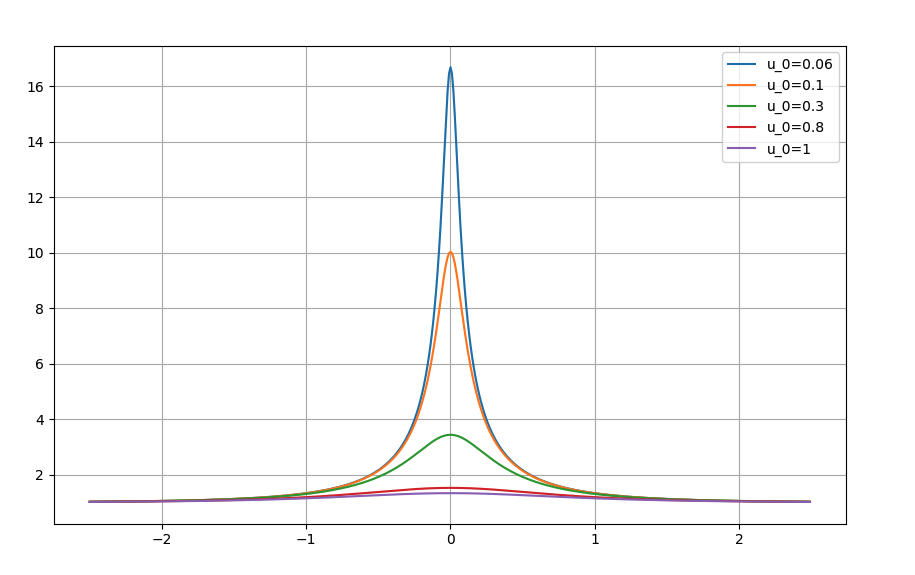
\includegraphics[scale=0.4]{ch13-p13.6.png}
\end{center}

\item [\textbf{c.}] Comparing the plotted curve on part \textbf{b.} with figure
13.6 we see that $u_0$ must be 0.06 and by taking the full with at half maximum
equal to 0.19 i.e. $\Delta t/t_E = 0.19$ we get that $t_E$ is
\begin{align*}
    t_E &= \frac{\Delta t}{0.19} =
    \frac{2~\text{days}}{0.19} = 10.52~\text{days}
\end{align*}
\end{itemize}
\end{proof}

\cleardoublepage
\begin{proof}{\textbf{P13.7}}
\begin{itemize}
\item [\textbf{a.}] We see that $dr/dt|_{r=r_0} = 0$ since $r$ has a
minimum at $r_0$ then equation (12.3) becomes
\begin{align*}
    1 &= \frac{b^2}{r_0^2}\bigg(1 - \frac{2GM}{r_0}\bigg)\\
    b^2 &= r_0^2\bigg(1 - \frac{2GM}{r_0}\bigg)^{-1}\\
    b &= r_0\bigg(1 - \frac{2GM}{r_0}\bigg)^{-1/2}
\end{align*}
\item [\textbf{b.}] We replace the value we have for $b$ in equation (12.3)
\begin{align*}
    % 1 = \bigg(1 - \frac{2GM}{r}\bigg)^{-2}\bigg(\dv{r}{t}\bigg)^2
    % + &\frac{r_0^2}{r^2}\bigg(1 - \frac{2GM}{r_0}\bigg)^{-1}\bigg(1 - \frac{2GM}{r}\bigg)\\
    1 - \frac{r_0^2}{r^2}\bigg(1 - \frac{2GM}{r_0}\bigg)^{-1}\bigg(1 - \frac{2GM}{r}\bigg)
    &= \bigg(1 - \frac{2GM}{r}\bigg)^{-2}\bigg(\dv{r}{t}\bigg)^2\\
    \bigg(1 - \frac{2GM}{r}\bigg)^{2}
    - \frac{r_0^2}{r^2}\bigg(1 - \frac{2GM}{r_0}\bigg)^{-1}\bigg(1 - \frac{2GM}{r}\bigg)^{3}
    &= \bigg(\dv{r}{t}\bigg)^2\\
    \bigg(1 - \frac{2GM}{r}\bigg)\sqrt{
    1 - \frac{r_0^2}{r^2}\bigg(1 - \frac{2GM}{r_0}\bigg)^{-1}\bigg(1 - \frac{2GM}{r}\bigg)}
    &= \dv{r}{t}\\
    \bigg(1 - \frac{2GM}{r}\bigg)\frac{1}{r}\sqrt{
    r^2 - r_0^2\bigg(1 - \frac{2GM}{r_0}\bigg)^{-1}\bigg(1 - \frac{2GM}{r}\bigg)}
    &= \dv{r}{t}
\end{align*}
Hence
\begin{align*}
    dt &= \frac{rdr}{\bigg(1 - \frac{2GM}{r}\bigg)\sqrt{
    r^2 - r_0^2\bigg(1 - \frac{2GM}{r_0}\bigg)^{-1}\bigg(1 - \frac{2GM}{r}\bigg)}}
\end{align*}
\item [\textbf{c.}] Let us ignore completely $2GM/r$ and $2GM/r_0$ then
equation (13.26) becomes
\begin{align*}
    dt &= \frac{rdr}{(1)\sqrt{r^2 - r_0^2(1)^{-1}(1)}} = \frac{rdr}{\sqrt{r^2 - r_0^2}}
\end{align*}
And by integration we get that
\begin{align*}
    t(r,r_0) &= \int_{r_0}^r \frac{rdr}{\sqrt{r^2 - r_0^2}}
    = \bigg[\sqrt{r^2 - r_0^2}\bigg]_{r_0}^r
    =\sqrt{r^2 - r_0^2}
\end{align*}

\cleardoublepage
\item [\textbf{d.}] Let us substitute $u = r/r_0$ and apply the binomial
approximation inside the square root as follows
\begin{align*}
    dt &= \frac{r_0udr}{\bigg(1 - \frac{2GM}{r_0 u}\bigg)\sqrt{
    r_0^2u^2 - r_0^2\bigg(1 + \frac{2GM}{r_0}\bigg)\bigg(1 - \frac{2GM}{r_0u}\bigg)}}\\
    &= \frac{udr}{\bigg(1 - \frac{2GM}{r_0 u}\bigg)\sqrt{
    u^2 - \bigg(1 + \frac{2GM}{r_0} - \frac{2GM}{r_0u}\bigg)}}\\
    &= \frac{udr}{\bigg(1 - \frac{2GM}{r_0 u}\bigg)\sqrt{
    u^2 - 1 - \frac{2GM}{r_0} + \frac{2GM}{r_0u}}}\\
    &= \frac{udr}{\bigg(1 - \frac{2GM}{r_0 u}\bigg)\sqrt{
    u^2 - 1 + \frac{2GM(1 - u)}{r_0u}}}\\
    &= \frac{udr}{\bigg(1 - \frac{2GM}{r_0 u}\bigg)\sqrt{
    (u^2 - 1)\bigg(1 + \frac{2GM(1 - u)}{r_0u(u^2 - 1)}\bigg)}}\\
    &= \frac{udr}{\bigg(1 - \frac{2GM}{r_0 u}\bigg)\sqrt{
    (u^2 - 1)\bigg(1 - \frac{2GM(u - 1)}{r_0u(u - 1)(u + 1)}\bigg)}}
\end{align*}
Let us also note that $dr = r_0du$ then
\begin{align*}
    dt &= \frac{r_0 udu}{\sqrt{u^2 - 1}\bigg(1 - \frac{2GM}{r_0 u}\bigg)\sqrt{
    1 - \frac{2GM}{r_0u(u + 1)}}}
\end{align*}

\cleardoublepage
\item [\textbf{e.}] Let us apply the binomial approximation on equation (13.27)
again to get
\begin{align*}
    dt &= \frac{r_0u}{\sqrt{u^2 - 1}}
    \bigg(1 + \frac{2GM}{r_0 u}\bigg)\bigg(1 + \frac{GM}{r_0 u(u + 1)}\bigg)~du\\
    &= \frac{r_0u}{\sqrt{u^2 - 1}}
    \bigg(1 + \frac{GM}{r_0 u(u + 1)} + \frac{2GM}{r_0 u}\bigg)~du
\end{align*}
Where we kept only first order terms. Now, by integration we get that
\begin{align*}
    t(1,u) &= \int_1^u 
    \frac{r_0u}{\sqrt{u^2 - 1}}
    + \frac{GM}{(u + 1)\sqrt{u^2 - 1}} + \frac{2GM}{\sqrt{u^2 - 1}}~du\\
    &= r_0\sqrt{u^2 - 1} + \frac{GM\sqrt{u^2 - 1}}{u + 1} 
    + 2GM\log(\sqrt{u^2 - 1} + u)\\
    &= r_0\sqrt{u^2 - 1} + GM\sqrt{\frac{(u - 1)(u + 1)}{(u + 1)^2}}
    + 2GM\log(\sqrt{u^2 - 1} + u)\\
    &= r_0\sqrt{u^2 - 1} + GM\sqrt{\frac{u - 1}{u + 1}}
    + 2GM\log(\sqrt{u^2 - 1} + u)
\end{align*}
Finally, substituting $u$ we have that
\begin{align*}
    t(r, r_0) &= \sqrt{r^2 - r_0^2} + GM\sqrt{\frac{r - r_0}{r + r_0}}
    + 2GM\log(\frac{\sqrt{r^2 - r_0^2} + r}{r_0})
\end{align*}

\cleardoublepage
\item [\textbf{f.}] The extra time a signal needs to get from Venus to earth
is 
\begin{align*}
    GM\sqrt{\frac{r_2 - r_0}{r_2 + r_0}} + 2GM\log(\frac{\sqrt{r_2^2 - r_0^2} + r_2}{r_0}) +\\
    + GM\sqrt{\frac{r_1 - r_0}{r_1 + r_0}} + 2GM\log(\frac{\sqrt{r_1^2 - r_0^2} + r_1}{r_0})
\end{align*}
Where $r_2 = 0.723~AU = 1.081 \times 10^8~km$, $r_1 = 149.6 \times 10^6~km$
and $r_0 = 696000~km$ then
\begin{align*}
    &1.477\cdot 0.9935 + 2\cdot 1.477 \cdot \log(310.62)
    + 1.477\cdot 0.9953 +\\
    &+ 2\cdot 1.477 \cdot \log(429.88) = 37.80~km = 126.08~\mu s
\end{align*}
\end{itemize}
\end{proof}

\cleardoublepage
\begin{proof}{\textbf{P13.8}}
\begin{itemize}
\item [\textbf{a.}] We assume all angles are small. We can approximate the
opposite side of the triangle formed by $\alpha_+$ with the horizontal by
\begin{align*}
    D_{LS}\tan\alpha_+ \approx D_{LS}\alpha_+
\end{align*}
This side must also be equal, by the same approximation, to
$$D_L \theta_+ - D_L \beta$$
Hence
\begin{align*}
    D_{LS}\alpha_+ &= D_L \theta_+ - D_L \beta\\
    \alpha_+ &= (\theta_+ - \beta)\frac{D_L}{D_{LS}}
\end{align*}
In the same way, the opposite side of the triangle formed by $\alpha_-$ with
the horizontal is given by $D_{LS}\alpha_-$ but also this side is
$$D_L |\theta_-| + D_L \beta$$
Hence
\begin{align*}
    D_{LS}\alpha_- &= D_L |\theta_-| + D_L \beta\\
    \alpha_- &= (|\theta_-| + \beta)\frac{D_L}{D_{LS}}
\end{align*}

\item [\textbf{b.}] From equation (13.14) we know that the angle the images
make with the line joining the earth and the lens object must be
$\theta_{\pm} = \frac{1}{2}(\beta \pm \sqrt{\beta^2 + 4\theta_E^2})$
then naming $\theta_0 = \frac{1}{2}\sqrt{\beta^2 + 4\theta_E^2}$ we get that
$$\theta_{\pm} = \frac{1}{2}\beta \pm \theta_0$$
Subtracting $\beta$ from both sides on the positive case we get that
\begin{align*}
    \theta_+ - \beta &= \frac{1}{2}\beta + \theta_0 - \beta\\
    \theta_+ - \beta &= \theta_0 - \frac{1}{2}\beta
\end{align*}
In the negative case we add on both sides $\beta$ to get what follows
\begin{align*}
    |\theta_-| + \beta &= \bigg|\frac{1}{2}\beta - \theta_0\bigg| + \beta\\
    |\theta_+| + \beta &= -\frac{1}{2}\beta + \theta_0 + \beta\\
    |\theta_+| + \beta &= \theta_0 + \frac{1}{2}\beta
\end{align*}

\cleardoublepage
\item [\textbf{c.}] The pathlength of the top light ray is given by the
sum of the hypotenuses of the two right triangles formed by the angles
$\alpha_+$ and $\theta_+ - \beta$. We can compute them using the cosine
of each angle i.e.
\begin{align*}
    \frac{D_{L}}{\cos(\theta_+ - \beta)} + \frac{D_{LS}}{\cos \alpha_+}
    = \frac{D_{L}}{\cos(\theta_0 - \frac{1}{2}\beta)}
    + \frac{D_{LS}}{\cos ((\theta_0 - \frac{1}{2}\beta) D_L/D_{LS})}
\end{align*}
Where we replaced what we computed on part \textbf{a.} and \textbf{b.}
Now using the first two terms of the cosine expansion in power series we get
that
\begin{align*}
    D_L\bigg(1 - \frac{\theta_0^2 - \beta\theta_0 + \beta^2/4}{2}\bigg)^{-1}
    + D_{LS}\bigg(1 - \frac{(\theta_0^2 - \beta\theta_0 + \beta^2/4)D_L^2}{2D_{LS}^2}\bigg)^{-1}
\end{align*}
But applying the binomial approximation we have that
\begin{align*}
    D_L\bigg(1 + \frac{\theta_0^2 - \beta\theta_0 + \beta^2/4}{2}\bigg)
    + D_{LS}\bigg(1 + \frac{(\theta_0^2 - \beta\theta_0 + \beta^2/4)D_L^2}{2D_{LS}^2}\bigg)
\end{align*}
On the other hand, for the bottom light ray, in the same way, we get that
\begin{align*}
    D_L\bigg(1 + \frac{\theta_0^2 + \beta\theta_0 + \beta^2/4}{2}\bigg)
    + D_{LS}\bigg(1 + \frac{(\theta_0^2 + \beta\theta_0 + \beta^2/4)D_L^2}{2D_{LS}^2}\bigg)
\end{align*}
Then subtracting both equations we get the difference $\Delta D$ betweeen
the pathlengths i.e.
\begin{align*}
    \Delta D  &= D_L\bigg(1 + \frac{\theta_0^2 + \beta\theta_0 + \beta^2/4}{2}\bigg)
    + D_{LS}\bigg(1 + \frac{(\theta_0^2 + \beta\theta_0 + \beta^2/4)D_L^2}{2D_{LS}^2}\bigg)\\
    &\quad- D_L\bigg(1 + \frac{\theta_0^2 - \beta\theta_0 + \beta^2/4}{2}\bigg)
    - D_{LS}\bigg(1 + \frac{(\theta_0^2 - \beta\theta_0 + \beta^2/4)D_L^2}{2D_{LS}^2}\bigg)\\
    &= D_L + \frac{(\theta_0^2 + \beta\theta_0 + \beta^2/4)D_L}{2}
    + D_{LS} + \frac{(\theta_0^2 + \beta\theta_0 + \beta^2/4)D_L^2}{2D_{LS}}\\
    &\quad - D_L - \frac{(\theta_0^2 - \beta\theta_0 + \beta^2/4)D_L}{2}
    - D_{LS} - \frac{(\theta_0^2 - \beta\theta_0 + \beta^2/4)D_L^2}{2D_{LS}}\\
    &= \beta\theta_0D_L +\beta\theta_0\frac{D_L^2}{D_{LS}}\\
    &= D_L\bigg(1 + \frac{D_L}{D_{LS}}\bigg)\beta\theta_0
\end{align*}

\cleardoublepage
\item [\textbf{d.}] The quasar is $D_{L} + D_{LS} = 8.7 \times 10^9~ly$
away from earth and the lensing galaxy is $D_L = 3.7 \times 10^9~ly$
from the earth, then $D_{LS} = 5 \times 10^{9}~ly$.

Also, since $\beta = 1.8 \theta_E = 1.944\times 10^{-5}~rad$ we get that
\begin{align*}
    \theta_0 = \frac{1}{2}\sqrt{
        (1.944 \times 10^{-5})^2 + 4(1.08\times 10^{-5})^2
    } = 1.453 \times 10^{-5}~rad
\end{align*}

So $\Delta D$ in this case is
\begin{align*}
    \Delta D &=
    3.7\times 10^9 \cdot \bigg(1 + \frac{3.7 \times 10^9}{5 \times 10^9}\bigg)
    \cdot 1.944 \times 10^{-5} \cdot 1.453 \times 10^{-5}\\
    &= 1.818~ly\\
    &= 664~\text{days}
\end{align*}
\end{itemize}
\end{proof}

\cleardoublepage
\begin{proof}{\textbf{P13.9}}
\begin{itemize}
\item [\textbf{a.}] The deflection angle of the sun for rays at the sun's radius
is
\begin{align*}
    \delta = \frac{4GM}{r} = \frac{4 \cdot 1.477}{696000}
    = 8.488505 \times 10^{-6}~\text{rad}
\end{align*}
Then by geometry (See FIG 13.4) we get that
\begin{align*}
    \tan(\frac{\pi}{2} - \delta) = \frac{D_L}{r}
\end{align*}
Hence
\begin{align*}
    D_L &= r\tan(\frac{\pi}{2} - \delta)\\
    &= 696000 \cdot \tan(\frac{\pi}{2} - 8.488505 \times 10^{-6})\\
    &= 81993236733.327~km\\
    &= 548.09~AU
\end{align*}
If we take a bigger radius (or impact parameter) then the angle $\delta$
decreases leading to a focus even further away. Therefore, it's better to put
the satellite farther from the sun.

\item [\textbf{b.}] Assuming we are imaging something infinitely far away 
we can take that $D_{LS} \approx D_S$ hence the Einstein angle is given by
\begin{align*}
    \theta_E = \sqrt{\frac{4GM}{D_L}} = \sqrt{\frac{4\cdot1.477}{81998114983.561}}
    = 8.488252 \times 10^{-6}~\text{rad}
\end{align*}
On the other hand the angular radius of the sun as seen from the satellite is
\begin{align*}
    \tan\theta \approx \theta = \frac{r}{D_L} = \frac{696000}{81998114983.561}
    = 8.488000 \times 10^{-6}~\text{rad}
\end{align*}
So the sun is going to be barely inside the Einstein ring.

\item [\textbf{c.}] We know that $1~ly = 9.461\times 10^{12}~km$ then Alpha
Centauri is at a distance of
\begin{align*}
    4.3~ly \cdot \frac{9.461\times 10^{12}~km}{1~ly}
    \cdot \frac{6.6846 \times 10^{-9}~AU}{1~km}
    = 271944.9~AU
\end{align*}
Then the angular separation between the star and the planet as seen from the
satellite is
\begin{align*}
    \tan\delta \approx \delta = \frac{1~AU}{271944.9~AU} = 3.67721\times 10^{-6}~\text{rad}
\end{align*}
Hence the planet is inside the Einstein ring.

\cleardoublepage
\item [\textbf{d.}]
Let us assume that $\beta \to 0$ i.e. the source is behind the sun with respect
to the spacecraft and they are almost aligned.
Then moving the spacecraft $1~km$ gives us
\begin{align*}
    D_L \beta &= 1~km
\end{align*}
Hence
\begin{align*}
    \beta &= \frac{1}{8.228 \times 10^{10}} = 1.2153 \times 10^{-11}~\text{rad}
\end{align*}
Using the sun as lens the intensity magnification is then
\begin{align*}
    \frac{I_{tot}}{I_s}
    &= \frac{1}{2}\bigg(\frac{\beta}{\sqrt{\beta^2 + 4\theta_E^2}}
    + \frac{\sqrt{\beta^2 + 4\theta_E^2}}{\beta}
    \bigg)\\
    &= \frac{1}{2}\bigg(
    \frac{1.2153 \times 10^{-11}}
    {\sqrt{(1.2153 \times 10^{-11})^2 + 4(8.488252 \times 10^{-6})^2}}\\
    &\quad
    + \frac{\sqrt{(1.2153 \times 10^{-11})^2 + 4(8.488252 \times 10^{-6})^2}}
    {1.2153 \times 10^{-11}}
    \bigg)\\
    &= 698413.37
\end{align*}

\item [\textbf{e.}] There will be only one image visible since the Einstein
ring is almost the size of the sun, hence the image inside the Einstein ring
will be blocked by the sun.

For the star $\beta$ is given by $\beta = \delta + \beta_{planet}$ where
$\delta$ is the angular separation between the planet and the star seen from
the satellite. Then the intensity magnification for the visible image of the
star is
\begin{align*}
    \frac{I_+}{I_s}
    &= \frac{1}{4}\bigg(\frac{\beta}{\sqrt{\beta^2 + 4\theta_E^2}}
    + \frac{\sqrt{\beta^2 + 4\theta_E^2}}{\beta} + 2
    \bigg)\\
    &= \frac{1}{4}\bigg(
    \frac{3.6772\times 10^{-6}}
    {\sqrt{(3.6772\times 10^{-6})^2 + 4(8.488252 \times 10^{-6})^2}}\\
    &\quad
    + \frac{\sqrt{(3.6772\times 10^{-6})^2 + 4(8.488252 \times 10^{-6})^2}}
    {3.6772\times 10^{-6}} + 2
    \bigg)\\
    &= 1.733
\end{align*}
Therefore, we don't need any shield for our detector since the
magnification of the star is significantly smaller compared to the planet's
magnification.

\item [\textbf{f.}] A 1-km shift of our spacecraft translates into a shift on
the planet's side of
\begin{align*}
    \beta D_S = 1.2153\times 10^{-11} \cdot 4.0682 \times 10^{13}~km = 494.4~km
\end{align*}
Where we used that $271944.9~AU = 4.0682 \times 10^{13}~km$.
\end{itemize}
\end{proof}
\end{document}